\section{涉众分析}

\subsection{什么是涉众}
涉众是指所有能够影响软件系统的实现, 或者会被实现后的软件系统所影响的个人和团体。

涉众分析围绕一个组织的各个部门内的员工所负责的业务展开
\begin{itemize}
    \item 所有的描述和胜败条件都和业务直接相关
\end{itemize}

此类涉众分析的难度随着组织机构的复杂性和不确定性增长而增加
\begin{itemize}
    \item 部门内$\rightarrow$部门间$\rightarrow$新业务部门$\rightarrow$组织间$\rightarrow$大众用户(互联网产品)
\end{itemize}


\subsection{涉众分析的过程}
涉众分析与前景与范围的定义是交织进行的,互为依赖
\begin{figure}[H]
	\centering
	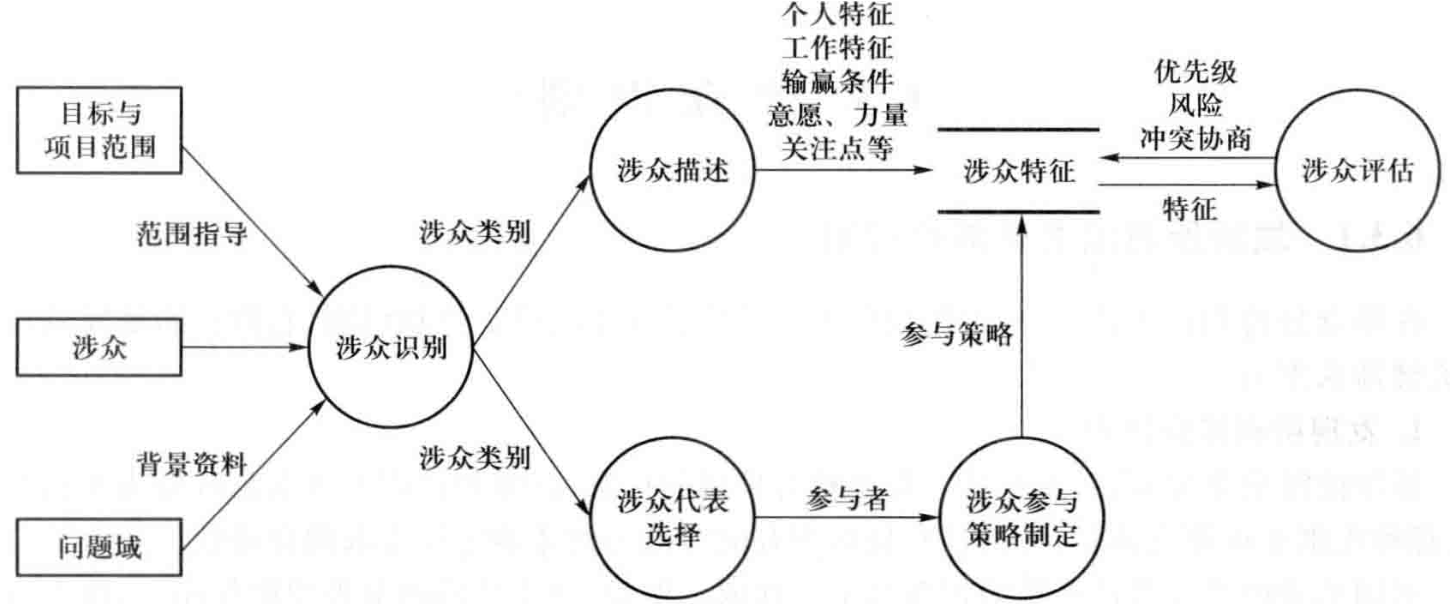
\includegraphics[width=0.85\textwidth]{img/涉众分析过程.png}
\end{figure}


\subsection{涉众识别}

\subsubsection{涉众识别的基本原则}
\begin{itemize}
    \item 涉众类别需要细分,发现所有类别
    \begin{itemize}
        \item 每一类涉众的所有成员都能够一致、稳定的从相同立场、相同视角来看待相同的软件系统
    \end{itemize}
    \item 发现比较关键的涉众
    \begin{itemize}
        \item 需要分析他们各自的赢利条件,以在相互妥协中尽力实现一个共赢的结局
    \end{itemize}
    \item 涉众群体不是固定不变的,需要持续维护
    \begin{itemize}
        \item 对涉众的理解不是一个完成之后就可以结束的活动,而是应该在完成之后继续保持适当的关注
    \end{itemize}
\end{itemize}

如果互动及其关注点属于项目的目标与范围,那么涉众就属于关键涉众
\begin{figure}[H]
	\centering
	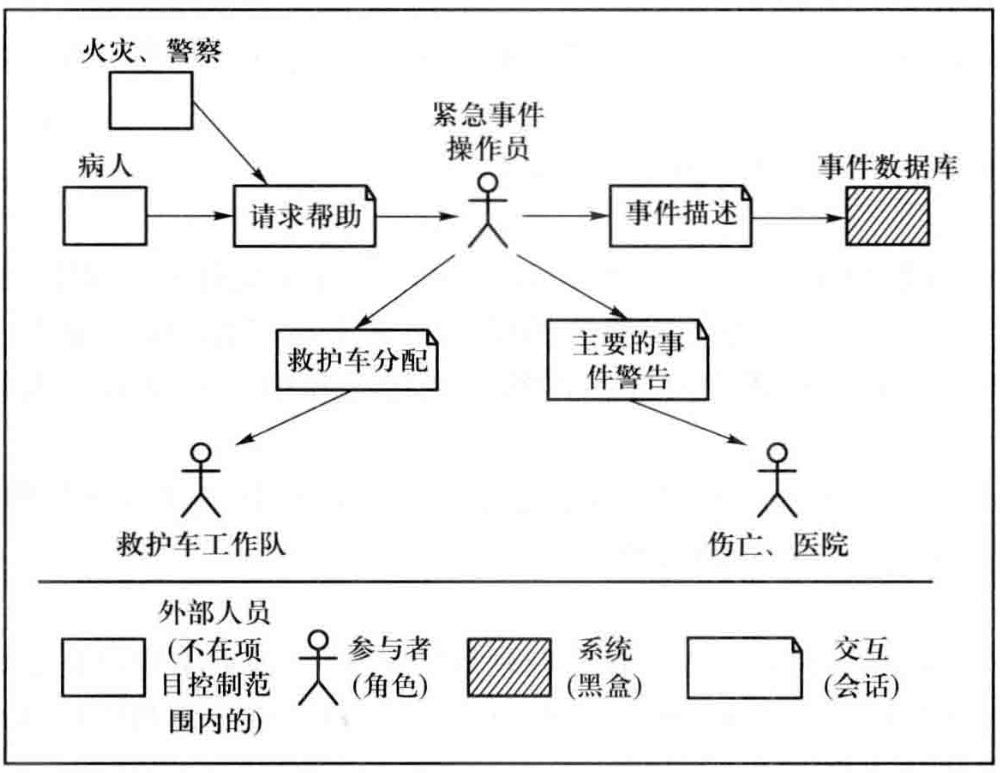
\includegraphics[width=0.65\textwidth]{img/救护车调度系统的交互网络草图.png}
    \caption*{救护车调度系统的交互网络草图}
    \vspace{-1em}
\end{figure}

\subsubsection{识别涉众的方法}
\begin{itemize}
    \item 简单方法:先膨胀后收缩方法
    \begin{itemize}
        \item 尽可能列出涉众后尝试合并,易用但可能有遗漏
    \end{itemize}
    \item 经典方法:涉众网络 方法
    \begin{itemize}
        \item 用容易发现的涉众(客户、管理者、投资人)出发
        \item 与初始涉众一起“膨胀—收缩”,集体确定关键涉众列表,再请列表中的新代表加入讨论,直到列表稳定
    \end{itemize}
    \item 经验方法:检查列表方法
    \begin{itemize}
        \item 在实践中人们总结出子常见的涉众类别列表,并据此指导涉众识别工作
    \end{itemize}
\end{itemize}

软件系统开发中常见的涉众类别有以下几种(检查列表方法)
\begin{itemize}
    \item 用户:最终使用和操作产品的人,关注软件功能 
    \item 客户:为软件系统的开发付费的人,关注经济上的成本、收益
    \item 开发者:负责实现软件系统的人,关注技术上的成本和收益
    \item 管理者:参与软件系统开发事务管理的人,投资方管理者、执行负责人、项目管理者,关注系统的开发进程
    \item 领域专家:在问题域中具有丰富知识的专家,关注软件中的知识(概括性、综合性) 
    \item 政府力量:法律法规、长远规划、政策意向等,起约束和指导作用
    \item 市场力量:组织中的市场部门人员,关注用户的想法
    \item 维护人员:系统的非功能属性,例如质量
\end{itemize}

利用\textbf{主体依赖模型}(Actor Dependency Model, ADM)分析涉众互动,识别关键涉众类别
\begin{itemize}
    \item 目标依赖(goal dependency):依赖者希望被依赖者满足一个条件,但不会规定怎样满足该条件。
    \item 软目标依赖(soft goal dependency):一种特殊类型的目标依赖,其条件是无法量化描述的。
    \item 任务依赖(task dependency):依赖者希望被依赖者执行特定任务。任务依赖比目标依赖更加具体,因为满足目标可以执行很多任务,被依赖者有自己的选择权。而任务依赖直接为被依赖者规定了任务。
    \item 资源依赖(resource dependency):依赖者希望被依赖者提供资源实体(抽象信息或者实物材料)为自己所用,但不关注提供资源需要被依赖者执行的行为和解决的问题。  
\end{itemize}
\begin{figure}[H]
	\centering
	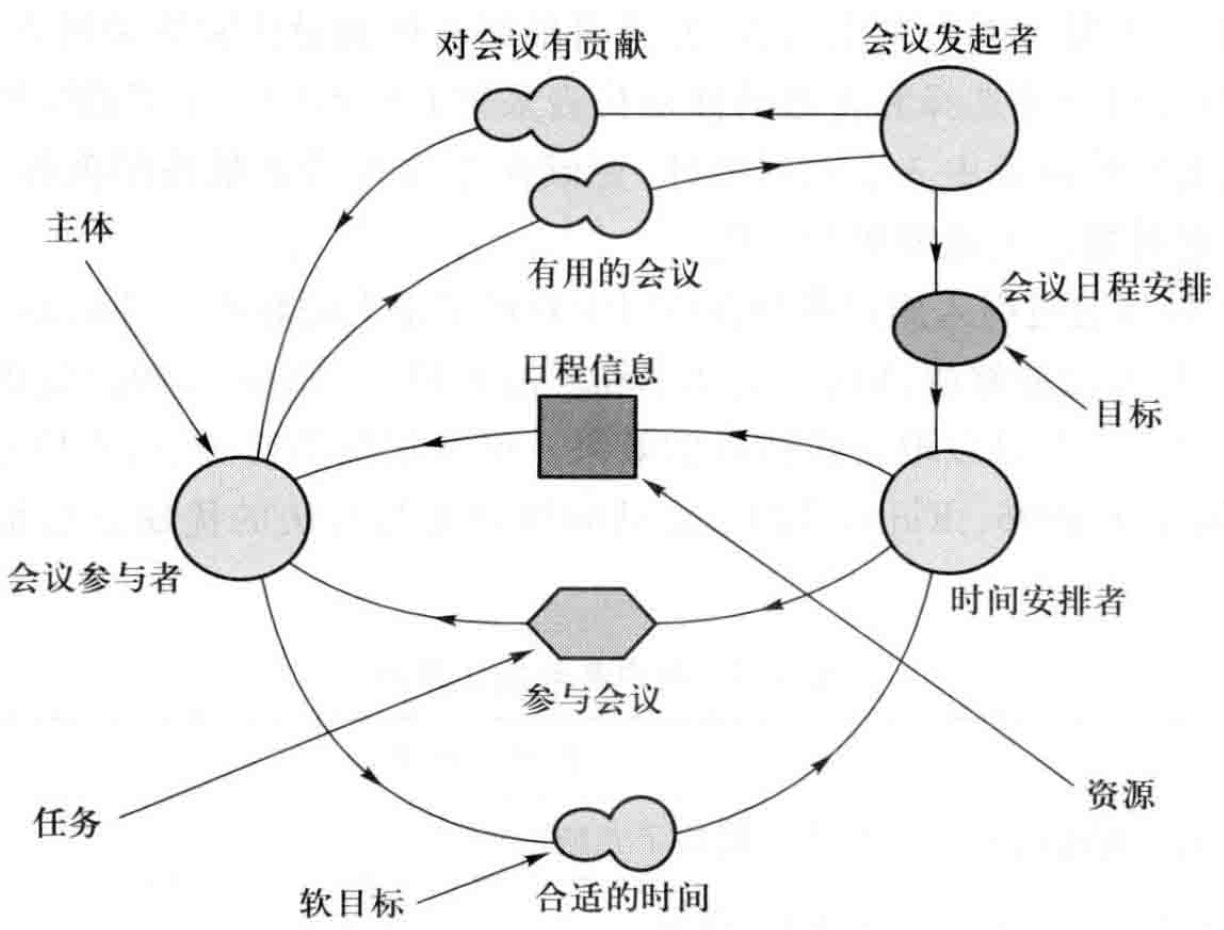
\includegraphics[width=0.7\textwidth]{img/主体依赖模型示例.png}
    \caption*{\textbf{主体依赖模型示例}}
    \vspace{-1em}
\end{figure}

\subsection{涉众描述}

\subsubsection{描述哪些内容}
\begin{itemize}
    \item L1:根据软件系统的功能前景寻找涉众
    \item L2:从涉众对象那里获取需求
    \item L3:分析涉众的输赢条件,实施共赢策略 
    \item L4:涉众对系统的影响力:了解涉众实现、监控和评估软件系统的能力,分析涉众的力量和影响范围;了解涉众实现、监控和评估软件系统的意愿,即分析涉众的关注点和兴趣取向
    \item L5:了解涉众的个人特征和工作特征,以便在涉众固定的情况下对软件系统的功能进行合理的调整  
\end{itemize}

\subsubsection{涉众简单特征描述}
涉众类别的特征描述
\begin{table}[H]
    \centering
    \begin{tabular}{|c|c|}
    \hline
    \multirow{4}{*}{个人特征}    & 年龄、性别、学历、职业、职务    \\ \cline{2-2} 
                             & 生活方式、个性、对新技术的态度   \\ \cline{2-2} 
                             & 技能                \\ \cline{2-2} 
                             & 身体能力及限制,例如色盲      \\ \hline
    \multirow{3}{*}{工作特征}    & 任务                \\ \cline{2-2} 
                             & 使用状况(利用程度、使用频率等)  \\ \cline{2-2} 
                             & 技能和经验(新手$\sim$专家) \\ \hline
    \multirow{3}{*}{地理和社会特征} & 地理:区域、国家          \\ \cline{2-2} 
                             & 文化背景              \\ \cline{2-2} 
                             & 社会关系              \\ \hline
    \end{tabular}
\end{table}

“化学制品跟踪系统”的涉众描述示例
\vspace{-0.8em}
\begin{center}
    \begin{longtable}{|Wc{3cm}|m{9cm}|}
        \hline
        涉众       & \multicolumn{1}{c|}{特征}                                                                               \\ \hline
        药剂师      & 药剂师将使用系统请求来自供应商和仓库的化学制品。药剂师每天多次使用系统,主要用于跟踪进出实验室的化学制品容器。药剂师需要在供应商目录中查找指定化学制品                                                                      \\ \hline
        采购者      & 采购者在采购部门处理其他用户所提交的化学制品请求,他们与外部的供应商建立联系,制定并发出订单。采购者对化学制品几乎不了解,因此将需要简单的查询机制来查找供应商目录。采购者不使用系统中容器跟踪这一特性。每个采购者平均每天使用系统10次                             \\ \hline
        化学制品仓库人员 & 化学制品仓库人员包括三个技师,管理着多达500 000种化学制品容器。他们将处理来自药剂师的请求并提供可用的容器,向供应商请求新的化学制品以及跟踪进出仓库的所有容器的流向,他们是货存清单和化学制品使用报告特性的唯一使用者。由于交易量大,化学制品仓库人员所使用的系统功能必须是自动化并且高效 \\ \hline
        卫生和安全人员  & 卫生和安全人员使用系统是为了生成符合官方关于化学制品使用和处理规则的季度报表。这些报表必须提前定义,并不需要特别查询能力,当官方的规则改变时,卫生和安全管理人员可能每年多次要求变化报表中的内容。报表变更优先级最高                                       \\ \hline
    \end{longtable}
\end{center}
\vspace{-3.7em}

\subsubsection{涉众深度信息描述}
\begin{itemize}
    \item 对项目的关注点和兴趣所在,态度是反对还是赞同
    \item 对项目的期望,成为项目赢家的条件
    \item 可能受到的项目的影响,影响的具体内容及影响程度
    \item 可以对项目施加的影响,力量的施加点及其强度
    \item 客户洞察中的移情图可以很好的补充涉众的深度信息  
\end{itemize}

自助餐厅在线订餐系统的涉众扩展特征描述
\vspace{-0.8em}
\begin{center}
    \begin{longtable}{|m{2cm}<{\centering}|m{2.4cm}|m{2.4cm}|m{2.4cm}|m{2.4cm}|}
    \hline
    涉众       & \multicolumn{1}{c|}{主要目标}                         & \multicolumn{1}{c|}{态度}                                             & \multicolumn{1}{c|}{主要关注点}                      & \multicolumn{1}{c|}{约束条件}                            \\ \hline
    公司管理层    & 提高员工生产率;节约自助餐厅的费用            & 强烈承诺完成版本2;如果有条件尽早完成版本3                         & 使用该系统所节约的费用必须超过开发和使用此系统的费用 & 无                               \\ \hline
    自助餐厅工作人员 & 更高效地利用了工作人员的整个工作时间;提高了客户的满意度 & 担心与工会的关系和可能的裁员,否则很愿意接受新系统                      & 保证工作                       & 培训工作人员使用Internet的技能;需要有送货的人员和车辆 \\ \hline
    顾客       & 可以更好地选择食物;节约了时间;更加方便         & 因为在自助餐厅和饭店就餐有社交作用,所以积极支持新系统,但使用系统的次数可能没有期望的次数多 & 使用要简单;送货可靠;食物选择要有效         & 需要访问公司的内部网络                     \\ \hline
\end{longtable}
\end{center}
\vspace{-3.7em}

\subsection{涉众评估}

\subsubsection{优先级评估}
\begin{itemize}
    \item (面向业务的)涉众并不是完全平等的,有些涉众比其他涉众更为重要
    \item 优先考虑涉众的基本特征,尤其是(涉众所完成的)任务特征 
\end{itemize}

一个医务(体检)软件的User/Task矩阵
\begin{table}[H]
    \centering
    \begin{tabular}{|c|c|c|c|}
    \hline
    用户群体 & 任务      & 群体数量 & 优先级 \\ \hline
    入院秘书 & 收集病人的数据 & 25   & 2   \\ \hline
    护士   & 查看体检信息  & 490  & 3   \\ \hline
    管理员  & 软件安装与维护 & 12   & 1   \\ \hline
    \end{tabular}
\end{table}


\subsubsection{风险评估}
\textbf{基于涉众特征与态度化解涉众风险策略}
\begin{itemize}
    \item 基于特征化解举例:亲子兴趣班
    \begin{itemize}
        \item 大人与小朋友一起参与:环境设定者(客户)$\rightarrow$ 参与者(用户)
        \item 良好的产品体验打造亲子品牌:被影响者(潜在用户/客户)$\rightarrow$ 参与者
    \end{itemize}
    \item 基于态度化解举例:电子竞技产业
    \begin{itemize}
        \item 与地方政府文化产业发展相结合:强反对者 $\rightarrow$ 强支持者
        \item 成功的赛事运营与未成年人游戏时长限制:弱反对者 $\rightarrow$ 弱支持者
    \end{itemize}
\end{itemize}

\begin{figure}[H]
	\centering
	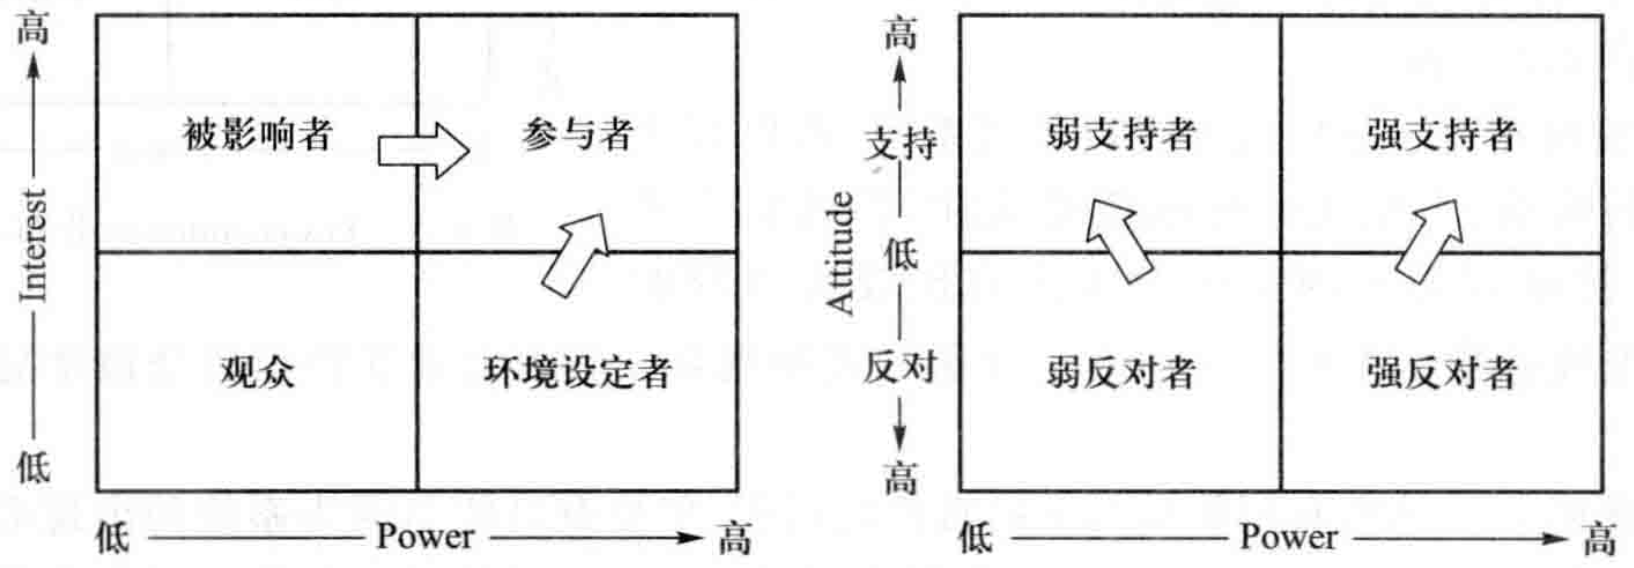
\includegraphics[width=0.8\textwidth]{img/化解涉众风险策略图.png}
    \caption*{\textbf{化解涉众风险策略图}}
    \vspace{-1em}
\end{figure}

\subsubsection{共赢分析}
\textbf{Stakeholder/Issue关系图}
\begin{itemize}
    \item 列出系统的所有涉众类别,明确描述他们的兴趣和对系统的期望
    \item 从涉众们的兴趣和期望中发现背后涉及的共同问题(Issue)
    \item 建立涉众类别和问题的关联,如果某个涉众类别对一个Issue存在兴趣,那么该涉众类别和这个Issue就存在关联关系
    \item 对每一个Stakeholder/Issue关系,标明该关系上面所被寄予的期望
\end{itemize}

\begin{figure}[H]
	\centering
	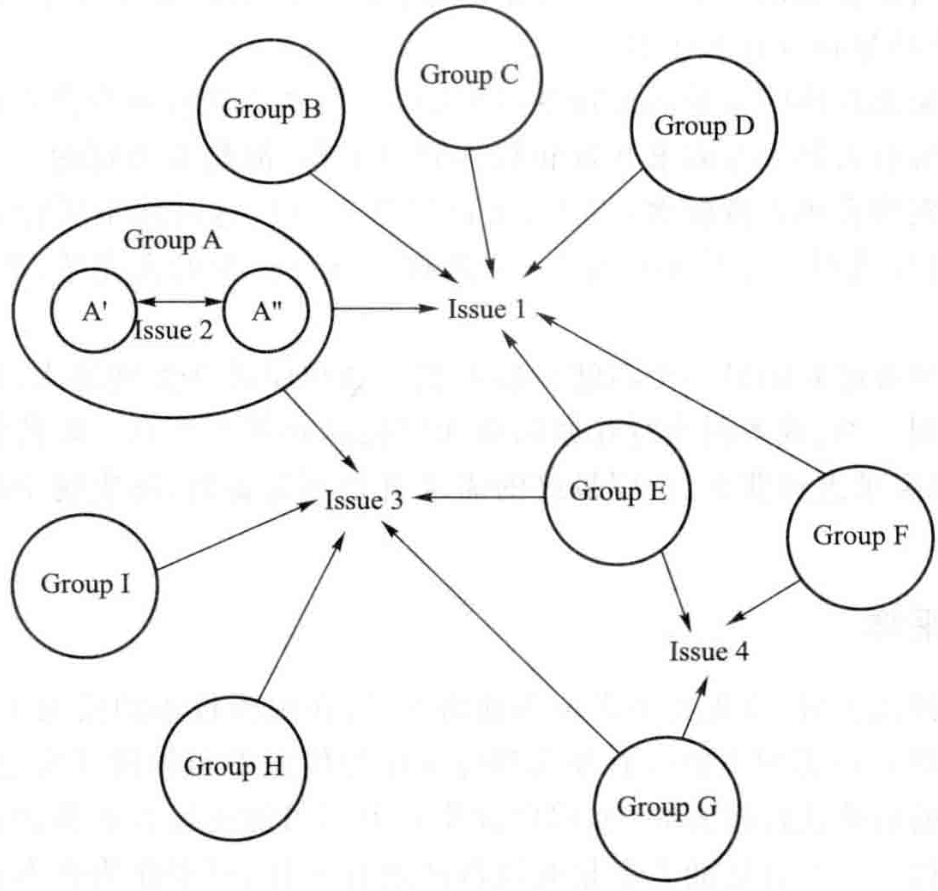
\includegraphics[width=0.5\textwidth]{img/Stakeholder-Issue关系图.png}
    \caption*{\textbf{Stakeholder/Issue关系图}}
    \vspace{-1em}
\end{figure}

基于Stakeholder/Issue关系图的共赢分析
\begin{itemize}
    \item 如果某个Stakeholder/Issue关系上所寄予的期望与项目的业务需求无法保持一致,那么它关联的涉众就在该Issue的问题上和项目整体目标存在冲突
    \begin{itemize}
        \item 涉众和项目负责人互相调整、折中 
        \item 重新评估项目的可行性 
    \end{itemize}
    \item 如果Stakeholder/Issue关系图中某个Issue所关联的不同关系标识有互相冲突的期望,那么就意味着它所关联的涉众在该Issue上存在需求冲突
    \begin{itemize}
        \item 分析各冲突方成为项目赢家的条件 
        \item 适当的调整,化解冲突 
        \item 分析项目在该Issue上的目标、约束和可选方案,并提供给冲突方进行权衡,促进他们之间协商解决   
    \end{itemize}
\end{itemize}

\subsubsection{利用目标模型深入评估涉众}
基于拥有者的目标模型,可以更好地执行涉众评估:
\begin{itemize}
    \item 将目标模型的目标配到主体
    \item 根据目标的优先级安排主体的优先级
    \item 根据目标的风险确定主体的风险
    \item 根据目标分析深入分析主体间的互动
    \begin{itemize}
        \item 根据目标冲突可以发现深层次的主体冲突
        \item 根据目标的冲突情况协商解决主体间的冲突
    \end{itemize}
\end{itemize}

\begin{figure}[H]
    \vspace{-0.5em}
	\centering
	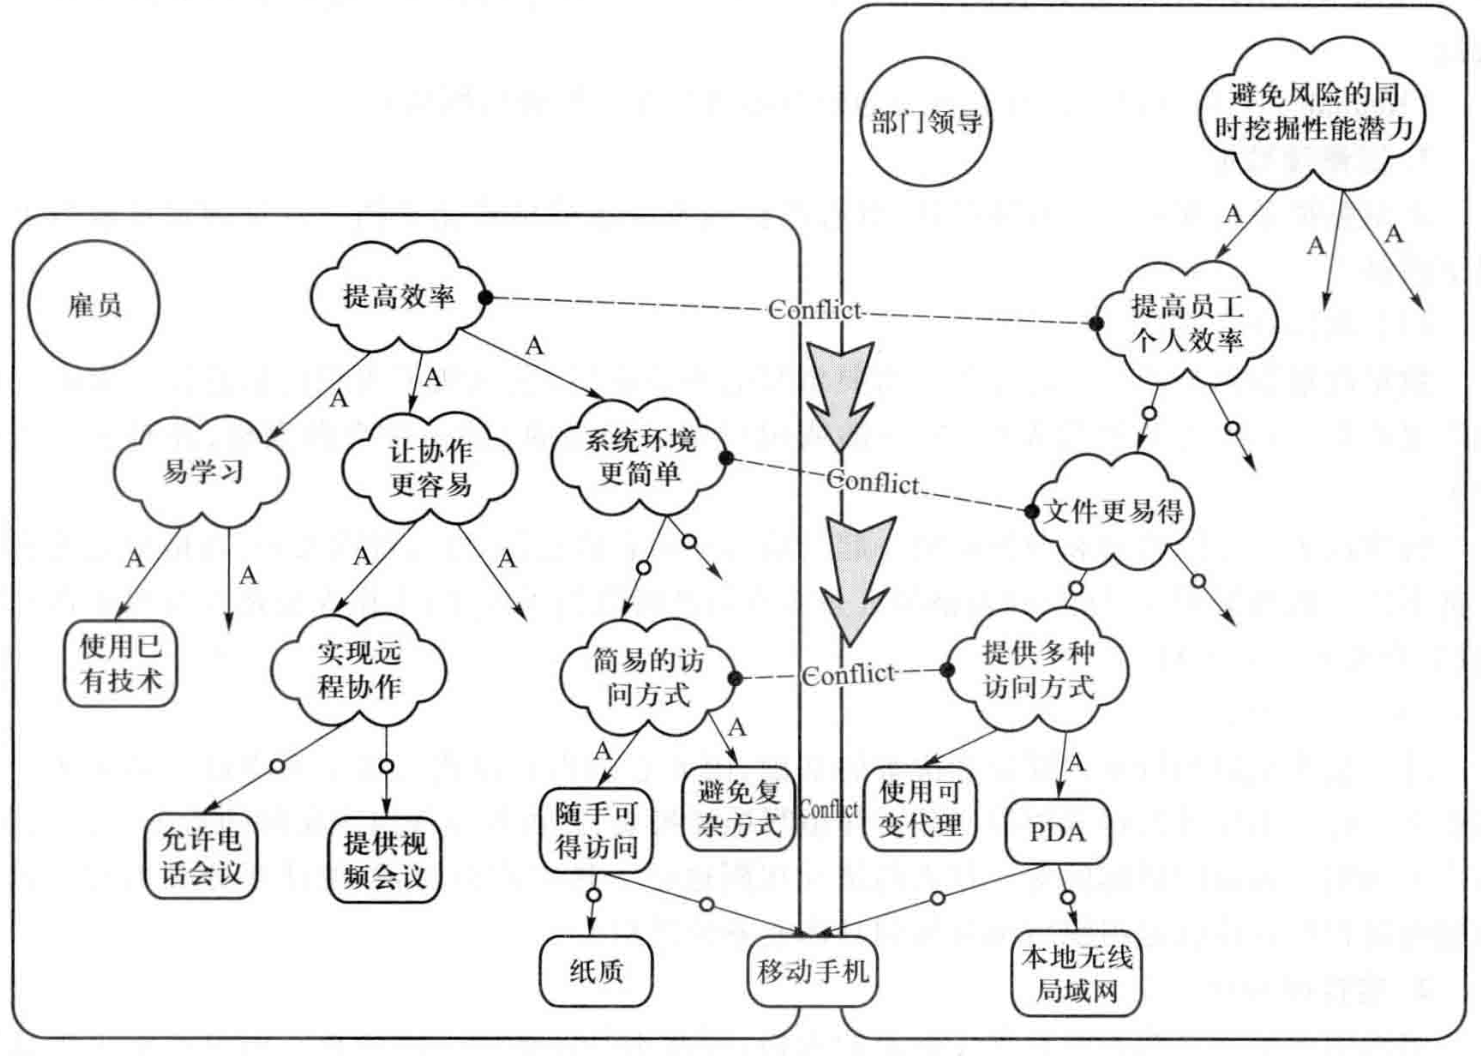
\includegraphics[width=0.68\textwidth]{img/拥有者的目标模型示例.png}
    \caption*{拥有者的目标模型示例}
    \vspace{-1.3em}
\end{figure}

\subsection{涉众代表选择}

\subsubsection{涉众采样}
\begin{itemize}
    \item 完整采样:每种涉众类别都有自己的代表
    \item 态度积极:愿意提供帮助
    \item 数量适中
    \begin{itemize}
        \item 太少:个人看法倾轧群体共同看法
        \item 太多:达成一致困难 
        \item 代表数量的准确数字要视项目的上下文环境来确定,一般为6$\sim$10
    \end{itemize}
    \item 比例恰当
    \vspace{-0.8em}
	\begin{multicols}{2}
        \begin{itemize}
            \item 计算机技能
            \item 业务技能
        \end{itemize}
	\end{multicols}
	\vspace{-1em}
\end{itemize}


\subsubsection{用户替代源}
在无法找到合适的涉众代表时,需求工程师可以考虑寻找一些涉众替代源——那些因为业务关系而和用户频繁接触的人。涉众替代源因为和用户在工作上存在频繁接触,所以能够较好地理解用户的真实想法,自然也就能够部分地代替他们发表看法。
\vspace{-0.8em}
\begin{multicols}{3}
    \begin{itemize}
        \item 市场人员
        \item 服务咨询人员
        \item 技术支持人员
        \item 领域专家
        \item (出色的)产品经理
    \end{itemize}
\end{multicols}
\vspace{-1em}

\subsection{涉众参与策略制定}

\subsubsection{制定涉众参与的基本策略}
代表们在合适的时间参与合适的工作
\begin{figure}[H]
    \vspace{-0.5em}
	\centering
	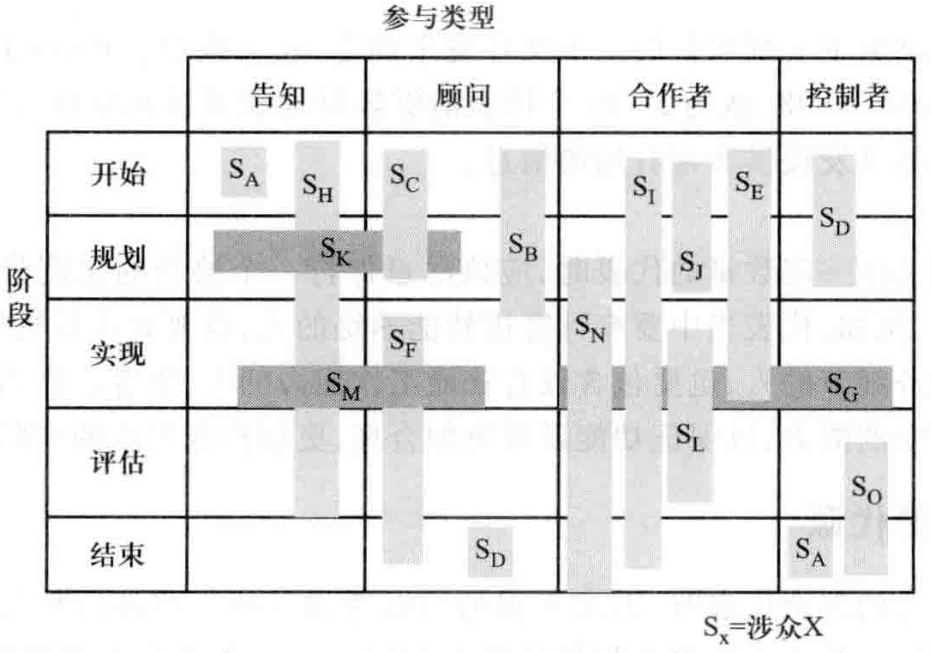
\includegraphics[width=0.6\textwidth]{img/涉众参与矩阵.png}
    \caption*{涉众参与矩阵}
    \vspace{-1em}
\end{figure}

\subsubsection{敏捷方法——用户参与}
\begin{itemize}
    \item 建立和用户的直接联系 
    \item 用户参与软件系统开发的整个过程 
    \item 反馈设计:最终的软件系统和用户的活动行为密切相关
    \item 主要通过社区来实现
\end{itemize}

用户参与的优缺点
\begin{table}[H]
    \centering
    \begin{tabular}{|c|l|}
    \hline
    \multirow{5}{*}{优点} & 会有更精确的用户需求,进而提高了系统的质量                                                             \\ \cline{2-2} 
                        & 可以避免发生代价昂贵的系统故障                                                                   \\ \cline{2-2} 
                        & 能提高用户对系统的接受度                                                                      \\ \cline{2-2} 
                        & 用户能够更有效的理解和使用系统                                                                   \\ \cline{2-2} 
                        & 可以提高组织内决策制定过程的参与度                                                                 \\ \hline
    \multirow{4}{*}{缺点} & 采集和管理巨量原始数据会花费很多时间                                                                \\ \cline{2-2} 
                        & 需要解决直接接触用户和对设计施加影响的困难                                                             \\ \cline{2-2} 
                        & \begin{tabular}[c]{@{}l@{}}用户通常不愿意在别人的观察下工作,而且研究\\ 发现用户在被观察时并不是真的在工作\end{tabular} \\ \cline{2-2} 
                        & 难以安排对用户工作过程的观察                                                                    \\ \hline
    \end{tabular}
\end{table}